\documentclass[12pt]{article}
%\documentclass[useAMS,usenatbib]{mn2e}
%\documentclass[apj]{emulateapj}

%%% TODO:
%1. fix numbers on numebrs.pro
%2. add table 1 and 2 (frac of barred galaxies and fraction fo galaxies barred
%3. fix figure 1.
%4 write results section
%5 write discussion section - add figute of 4 plots conclusions,etc.

%\voffset-1.25cm
\newcommand\ion[2]{#1$\;${\scshape{#2}}}%                       % ion, i.e., CII = \ion{C}{ii}
%\setlength{\textwidth}{6.5in} 
%\setlength{\textheight}{8.5in}
%\setlength{\topmargin}{-0.0625in} 
%\setlength{\oddsidemargin}{0in}
%\setlength{\evensidemargin}{0in} 
%\setlength{\headheight}{0in}
%\setlength{\headsep}{0in} 
%\setlength{\hoffset}{0in}
%\setlength{\voffset}{0in}



\usepackage{graphicx,natbib,times}
\usepackage{deluxetable} 


%\title[Galaxy Zoo: Bars and AGN ]{Galaxy Zoo: Bars as evidence of secular evolution in AGN host galaxies
%\thanks{This publication has been made possible by the participation of more than 300,000 volunteers in the Galaxy Zoo project. Their contributions are individually acknowledged at \texttt{http://www.galaxyzoo.org/Volunteers.aspx}.}}
%\author[Cardamone et al.]{
%  \parbox[t]{16cm}{
%Carolin Cardamone$^{1,2}$\thanks{ccardamone@astro.yale.edu},
%Kevin Schawinski$^{2,3}$, et al.
%Marc Sarzi$^{4}$,
%Steven P. Bamford$^{5}$,
%Nicola Bennert$^{6}$,
%C. M. Urry$^{2,3}$,
%Chris Lintott$^{7}$,
%William C.  Keel$^{8}$,
%John Parejko$^{9}$,
%Robert C. Nichol$^{10}$,
%Daniel Thomas$^{10}$,
%Dan Andreescu$^{11}$,
%Phil Murray$^{12}$,
%M. Jordan Raddick$^{13}$,
%An\v{z}e Slosar$^{14}$,
%Alex Szalay$^{13}$,
%Jan VandenBerg$^{13}$
%  }\\
%$^{1}$Astronomy Department, Yale University 208121, New Haven, CT 06520, U.S.A.\\
%$^{2}$Yale Center for Astronomy and Astrophysics, Departments of Physics and Astronomy, Yale University, New Haven, CT 06520, USA \\
%$^{3}$Department of Physics, Yale University, P.O. Box 208121, New Haven, CT 06520, USA. \\
%$^{4}$Centre for Astrophysics Research, University of Hertfordshire, College �Lane, Hatfield, Herts AL10 9AB, UK.\\
%$^{5}$Centre for Astronomy and Particle Theory, University of Nottingham, University Park, Nottingham, NG7 2RD, UK.\\
%$^{6}$Department of Physics, University of California, Santa Barbara, CA 93106, USA. \\
%$^{5}$Department of Physics, University of Oxford, Oxford OX1 3RH, UK.\\
%$^{8}$Department of Physics and Astronomy, University of Alabama, Tuscaloosa, AL, 35487, USA. \\
%$^{9}$ Department of Physics, Drexel University, Philadelphia, PA 19104, USA. \\
%$^{10}$Institute of Cosmology \& Gravitation, University of Portsmouth, Portsmouth, PO1 2EG, UK. \\
%$^{11}$LinkLab, 4506 Graystone Ave., Bronx, NY 10471, USA. \\
%$^{12}$Fingerprint Digital Media, 9 Victoria Close, Newtownards, Co. Down, Northern Ireland, BT23 7GY, UK.\\
%$^{13}$Department of Physics and Astronomy, The Johns Hopkins University, Baltimore, MD 21218, USA.\\
%$^{14}$Berkeley Center for Cosmological Physics, Lawrence Berkeley National Lab, 1 Cyclotron Road, MS 50-5005, Berkeley, CA 94720, USA\\
%}

%\date{In Prep, version April 09}
%\newcommand\aj{{AJ}}
%\newcommand\araa{{ARA\&A}}
%\newcommand\apj{{ApJ}}
%\newcommand\apjl{{ApJ}}
%\newcommand\apjs{{ApJS}}
%\newcommand\aap{{A\&A}}
%\newcommand\nat{{Nature}}
%\newcommand\mnras{{MNRAS}}
%\newcommand\pasp{{PASP}}

%\pagerange{\pageref{firstpage}--\pageref{lastpage}} \pubyear{2009}

%\def\LaTeX{L\kern-.36em\raise.3ex\hbox{a}\kern-.15em
%    T\kern-.1667em\lower.7ex\hbox{E}\kern-.125emX}

%\newtheorem{theorem}{Theorem}[section]

\begin{document}
%\title{Galaxy Zoo: Environment of Peas }
\noindent {\LARGE Galaxy Zoo: The Environments of the Peas}

%\label{firstpage}

%\maketitle

\begin{abstract}
\end{abstract}
%\begin{keywords}
% galaxies: evolution, galaxies: formation, galaxies: starburst, galaxies: dwarf, galaxies: high-redshift, galaxies: Seyfert
%\end{keywords}

\section{figures}


\section{Introduction}
\label{sec:intro}
This memo contains  Figures / Tables made in the GZ investigation into the environment surrounding green pea galaxies.   Along the way, a search is made to update our catalog of 'green peas' and investigate the initial search parameters characterizing the hunt for Peas.
 
Low mass starforming galaxies are thought to be the building blocks of galaxies, playing an important role in early galaxy assembly and evolution \citep{Pillepich2015}.
`Green Peas' or `Peas' were galaxies first discovered in the Galaxy Zoo Survey, due to their small and green appearance in the SDSS images.
Followup studies have shown them to be examples of relatively lower-mass, highly starforming galaxies, perhaps analogous to SF episodes occurring in the early universe.
The question we wish to investigate is do the peas have a 'typical' environment
 
Encoded in the large scale structure of the Universe, is a variety of cosmological parameters as well asn key infomraiton about the physical processes which underpin the formation of cosmic structures.
Heirchrical structure formation, our current paradigm of galaxy formation, places they a key role on gravititaion evolution of dark matter clustering around intial peaks providing potential werlls for gas halows and galxies to form in.
 
 
% Note scale at 0.112 is 2.068 kpc/", 12.253 Gyrs and scale at 0.360 is 5.078 kpc/", 9.734 Gyrs)
%$4.226 kpc/" = 4226 pc/" = 0.004226 Mpc/"$, so 1 Mpc at this redshift is 236" on an image or 4 arc minutes.
%Angular size distance = transverse size/theta angle (in radians)
%So at 0.275, D_A is 871.7 Mpc, meaning 1 radian would cover 871.7 Mpc on the sky, OR 206265 arcseconds=871.7 Mpc, or 1 arcseconds is 0.004226 Mpc.  
%A  galaxy is 1-10 kpc , 0.001-0.01 Mpc or .2-2 arcseconds in diameter on the image at that redshift
%A galaxy cluster diameter is 2-10 Mpc
%%%(Previous calculation 1.8" is roughly 8 kpc at 0.2832)
%25 arcseconds is 5 mpc/.1995
Cardamone et al 2009 leveraged a sample of 251 colour-selected galaxies in SDSS DR7 using a series of color cuts at $0.112<z<0.360$, where the OIII line falls in the r-band filter,  to define the original sample of `pea' galaxies.  
A final cut produced 80 confirmed peas after fitting the spectra for confirmation of star formation driving the emission.


At that time, using counts of projected neighbors to the original sample.  

\begin{figure}[h]
\begin{center} %NOTE compile with TEX & DVI
%\includegraphics[width=0.5\textwidth, angle=180]{pea_n1Mpc_ks.pdf}
\end{center}
\caption{\small{ Figure 3 from Cardamone et al. 2009 (made by Stephen Bamford).  The cumulative distribution of neighbour counts for the Peas
(solid line) is significantly different than a comparison galaxy sample (dotted line). No Peas live in the highest density environments.
}}
\label{fig:orig}
\end{figure}

Now return using 

The clustering of a set of galaxies can provide statistical measure of the average environment in which they live.  As a galaxies 

We adopt a $\lambda$CDM cosmology with 
$H_0 = 71  \: {\rm km \: s^{-1} \: Mpc^{-1}}$, $\Omega_{\rm m} = 0.3$ and $\Omega_{\rm \lambda} = 0.7$. 
\section{Data}
\subsection{Green Pea Galaxies}
The original sample of 80 confirmed peas was derived from DR7 after fitting the spectra for BPT Star Forming Galaxies from a sample within the color space (above) and $0.112<z<0.360$, where the OIII line falls in the r-band filter.  The main goal of Cardamoneetal2009 was to select a uniform sample of objects that could be investigated to uncover their properties.  The redshift range was selected so that the OIII line fell within the r-band filter (providing the 'green' appearance in the SDSS images) and a color selection region was defined to avoid sequences of galaxies and QSOs.  There is no uniform selection for the objects throughout the SDSS footprint,  as we look for Peas only in the spectroscopic sample of objects and keep them only in objects with classified as Starforming with spectral line amplitude over noise (AON) $\ge 3$ in all 4 lines in the BPT diagnostic. 
 In this paper, our goal is to quantify the environments in which these galaxies live.  In order to study this we take advantage of the huge expansion of SDSS spectroscopy through DR13, and use this to expand our sample of Peas.   

Starting with the simple color-selection region within the redshifts $0.112<z<0.360$, DR13's PhotoObjAll catalog provides a sample of 4155 galaxies, which could be nominally labeled as 'pea' colored.  This sample also includes the requirement's of a PSFMAG\_R $\ge 10$ and PETRORAD\_R $\le 5$.  However, DR13's PhotoObjAll catalog contains numerous interloping objects (from artifacts, small regions of larger galaxies, and other objects with bad photometry).  We wish to again select a catalog of Star Forming Peas, compact and with OIII emission powered by star formation.  To recover this sample, we require spectral line measurements and therefor use the catalog provided by the Portsmouth Group in DR12, which uses the same programs we used for the original sample (Penalized PiXel Fitting (pPXF, Cappellari and Emsellem 2004) and Gas and Absorption Line Fitting code (GANDALF v1.5; Sarzi et al. 2006)) to derive emission line properties \citep{Thomas2013}.
 Looking at images of the galaxies, shows many interloping objects which do not physically appear as peas.  Of the objects in the color-redshift space, 2203 have spectral fits in the Portsmouth catalog.   Many have non-starfomring BPT diagnostics, including 213 Seyfert galaxies, 65 LINERa, and another (52+103+87= 242) composite spectra.   Selecting for starforming objects only, leaves a sample of 1592 objects.  Requiring clean photometry (SDSS flag CLEAN=1, removing objects with deblending issues, those on plate edges, etc.), leaves 1454 objects. Of the 138 objects with the Clean flag =0, there are perhaps a dozen that look like clean peas on the image.  If we wish to limit the sample to those with individual $AON>3$ in each of the special line measurements, only 739 objects remain.  For the initial purposes of the clustering measurements - we'll use the full sample.


\begin{figure}[h]
\begin{center} %NOTE compile with TEX & DVI
%\includegraphics[width=1\textwidth, angle=90]{peaphotflag0.ps}
\end{center}
\caption{\small{ Phot Flag 0 sample of objects, removed from the spectroscopic sample eventhough classified as SF.  Of the 138 objects with the Clean flag ne 1, there are perhaps a dozen that look like clean peas on the image.  
}}
\label{fig:orig}
\end{figure}



\subsection{Luminous Red Galaxies}
Luminous Red Galaxies represent a sample of passive, massive early-type galaxies (Eisenstein et al. 2001) extending over a redshift range $0.16 \le z \le 0.7$ in SDSS much further than the main galaxy sample (Strauss et al. 2002).
Samples from SDSS have been used for a variety of studies from baryon acoustic oscillations (Kazin et al. 2010) to clustering (Padamanabhan e t al. 2009) and redshift space distortion studies (Hikage and Yamamoto 2013).
Classic samples of LRG were targeted as part of the SDSS-I and SDSS-II programs (Eisenstein et al. 2001) and from SDSS-III as part of the Baryon Oscillation Spectroscopic Survey program (Dawson et al. 2013).
Luminous Red Galaxies are well suited for tracing dark matter distribution and a useful comparison for cross-correlations due to their intrinsic brightness and relatively high spacial density (Einstein et al. 2001; Wake et al. 2006).

% Padmanabhan et al. 2009; Reid & Spergel 2009; Parejko et al. 2013
The clustering properties of LRGs have been used to constrain cosmological parameters (e.g., Tegmark et al. 2004) as well as measuring baryon acoustic oscillation scales (Eisenstein et al. 2005, Anderson et al. 2012).
Halo Occupation Distribution models have been shown to be a good representation for the autocorrelation function of the Luminous Red Galaxies measured from SDSS (Zehavi et al. 2005; Reid \& Spergel 2009; White et al. 2011).
This modeling work shows that LRGs reside in massive halos with $M\sim 10^{13} h^{-1}M_/sun$ and parent dark matter halos with masses of $M\sim 10^{15} h^{-1}M_/sun$ can host several LRGs (Masaki et al. 2013).

%The original sample of Luminous Red Galaxies from SDSS was selected using a series of magnitude and color-cuts.  We select a sample of galaxies from DR13, following a similar series of cuts ({$http://skyserver.sdss.org/dr12/en/help/docs/realquery.aspx\#lrg$}), and search the SpecObjAll catalog for matching bestObjIDs.  This sample returns 307252 objects of whom 210786 have a labeled source type of 'LRG' identified as the primary target for the legacy spectral observation.  If we look in the redshift range of our peas $0.112<z<0.360$, there are 168362 LRGs.  However, it's worth noting that only 10k of these are below the median pea redshift ($z\sim0.26$).

For our analysis we use the BOSS DR12 Galaxy Catalog (Alam et al. 2015, Eisenstein et al. 2011) LOWZ sample of Luminous Red Galaxies \citep{Reid2016}  and the associated randoms catalog.


\section{Clustering}

For our new-expanded sample of Peas, we can compute a three-dimensional correlation function.  However, even with our order of magnitude larger expanded sample of Peas, small number statistics limit the accuracy with which we can determine correlation functions, particularly in the case of autocorrelation functions.  Cross-correlation functions can utilize higher space density samples of objects in similar sky and redshift space as our Peas.  Luminous Red Galaxies low-z sample is good for this.  Cross correlating samples of lower-density objects with dense galaxy samples tracing the large scale structure in the field can lead to lower statistical errors than measuring the autocorrelation function directly.  Additionally, using cross-correlation functions does not require a complete understanding of the selection function of the galaxy sample of interest, which may not be well understood.  INstead, we can leverage a well determined selection function for the galaxy tracer sample.

To interpret a correlation function, a large scale bias measure can be computed for linear growth and biasing schemes - this will only be accurate for correlation function measurements on larger scales ($\sim1-2 h^{-1}$ Mpc). 
In order to more accurately explore the correlation function's measurements, a Halo Occupation Distribution framework can be used to constrain how various galaxy samples are distributed among dark matter halos - in particular explore both their presence as centers and/or satellite galaxies n the dark matter halos.
To compute a correlation function, a random sample must be generated for comparison to each dataset, accounting for any variations in detection limits.
To generate the random catalog for the Peas, we drew redshifts from the Pea-redshift distribution and randomized their location in RA and Dec by adding or subtracting up to a degree from their positions.
$\xi$ was determined using the pair counter from CorrFunc (Manodeep et al.) in bins of distance perpendicular to the line of site $r_p$ and parallel to the line of site $\pi$.
For catalog's like the peas, it is simple to use a KDE gaussian kernel to smooth their z distribution along the line of sight.  However, it is far more complicated in terms of RA/DEC position.  Not all objects in the photometric catalog that fit a pea's color, shape, etc. received redshift measurements.  In fact, most 'peas' selected received an extra fiber available in the field and were  thus marked as a 'serendipitous source'.

\subsection{Two Point Correlation Function $\xi$}

The two point correlation function (xi, $\xi$) quantifies the excess probability (relative to a Poisson distribution) of finding pair of galaxies at a given distance (r) from each other in a given volume element $dV$. Peebles 1980 expresses this given a mean number density of galaxies $n$ as:
\begin{equation}
dP=n[1+\xi(r)]dV
\end{equation}
As the RA and Dec of the objects are known to a great degree of accuracy the angular two-point correlation function ($w(\theta)$) can be computed to determine the conditional probability of finding a galaxy within a solid angle d$\Omega$ at an angle $\theta$ from another galaxy.
% https://ned.ipac.caltech.edu/level5/March04/Jones/Jones5_2.html
With the additional information provided by redshifts, real-space or 3D correlation functions can be computed.
However, projected distances (in RA/Dec) have greater accuracy than those along the line of sight because the redshifts will be distorted due peculiar motions (Fisher 1994). 
Therefore the spatial correlation function is typically split into a projected co-moving dimension along the line of sight $\pi$ and perpendicular to it $r_p$.  
The projected correlation ($w(p)$) function along a line of site can be determined to integrate over individual redshift-space distortions along the line of sight (Davis \& Peebles 1983).
\begin{equation}
w_p(r_p)=2 \int_{0}^{\pi_{max}} \xi(r_p,\pi) d\pi
\end{equation}

The correlation function can be represented as a power law with the 3D correlation slope $\gamma$ and correlation length $r_0$.
\begin{equation}
\xi(r)=(\frac{r}{r_0})^{-\gamma}
\end{equation}
And the projected correlation function can be represented as 
$w(r_p)= \Gamma(1/2) \Gamma[(\gamma-1)/2] / \Gamma(\gamma/2) r_0^\gamma r_p^{1-\gamma}$ (Peebles 1980).
At larger scales, typically $r_p \ge 1-2$ Mpc/h, the amplitude of the correlation function ($w_p(r_p)$) is due to the correlation between objects in distinct halos.
This linear regime is well modeled by the power law fit and the bias parameter represents the relationship between the large-scale clustering amplitude of the correlation function of the data and the 2-halo term for the dark matter distribution.
\begin{equation}
b_{2h}=\sqrt{\frac{w_{p,2h}(r_p)}{w_{DM,2h}(r_p)}}
\end{equation}
Computing this requires determining a dark matter projected correlation function.a


The bias can be related to the halo mass (van den Bosch 2002) Sheth et al. 2001 through a bias-mass relation $b(M_h,z)$.  The clustering and number density of a given halo is determined by its mass.  
Analytically this is characterized by the amplitude of density fluctuations from which a halo of mass $M_h$ forms at a given redshift ($\nu=\delta_c/\sigma(M_h,z)$).  The halo bias can then be modeled a function of halo masses or a fixed redshift (see e.g., \citep{cappelluti2012}, \citep{allevato2016}).


The mass of a halo is related to it's clustering and the number of hals
http://adsabs.harvard.edu/abs/2002MNRAS.331...98V

The two-point correlation function is most determined using a comparison to a random sample (pure noise) to see the strength of the signal at any given distance.   The Landy-Szalay  estimator is commonly used today, as it has been shown to provide the smallest statistical variance (Fisher 1994) and to be more accurate at larger scales (PonsBorderia et al. 1999, Kerscher et al. 2000). 
Given the Peas sample ($D_1$ ), a comparison galaxy sample ($D_2$) and matched samples randomized in locations ($R_1$,$R_2$) the Landy-Szalay estimator is:
\begin{equation}
\xi(r) = \frac{D_1D_2(r) - D_2R_2(r)-R_1D_2 + R_1 R_2(r)}{R_1 R_2 (r)}
\end{equation}
In this fucntion, each pair corresponds to pairs of objects with a given separation (e.g., $D_1 D_2(r)$ is the number of pairs between the galaxy and pea catalogs with a distance r).
However, this measurement of the correlation function requires the construction of an accurate estimate of the distribution function to create matched random catalog for each data set, reproducing the data's selection function and observational limitations.
The estimate of $\xi(r)$ is strongly dependent on the accuracy from which selection effects are reproduced including flux limits and optical followup limitations (the mask effect).  
Given the non-uniform selection of the Peas, it is not possible to estimate an accurate detection map projected on the sky from which the random distribution can be drawn.
Lacking the necessary projected detection distribution for deriving an accurate randoms catalog, Padamanabhan et al. 2009, used a the Peebles estimator estimator for a quasar function:
\begin{equation}
w_\theta(R) = \frac{D_{1}D_{2}}{D_{1}R_{2}}-1
\end{equation}
(Davis and Peebles 1983).
An accurate estimate of the distribution of random samples is necessary to compute a correlation function.




However, a better interpretation fits an empirical model relating the galaxies to their dark matter halo with a statistical model of the clustering of galaxies within a given dark matter halo.  This transforms pair counts of galaxies into a more physically informative relationship between the galaxies and the dark matter halo in which they reside.

\subsection{Halo Model}
To interpret large-scale clustering data, the relationship between the galaxies themselves and their dark matter halo hosts must be modeled.
The Halo Occupation Distribution is an empirical model that associates the galaxies in the data with dark matter halos as a function of the mass of the dark matter halos (Peacock \& Smith 2000).  
This approach first models a distribution of halos from a given cosmological model and then populates the galaxies of interest into the dark matter halos resulting in a probability that a halo of mass $M_h$ contains N objects of a particular type - $P(N|M_h)$ the halo occupation distribution function.
To determine the HOD we can model the two-point projected correlation function as a sum of two terms, a 1-halo term (1h) where both objects occupy the same dark matter halo and a 2-halo term (2h), where each pair of objects occupy a different dark matter halo.
\begin{equation}
w_p(r_p)=w_{p,1h}(r_p)+w_{p,2h}(r_p)
\end{equation}
Applying a predefined functional form to this relationship, allows 
To fit a measured correlation function, we can parameterize the Halo Occupation Distribution (as a sum of the number of central and satellite galaxies) and adopt a cosmology.
\cite{Zheng2009} Zheng et al. (2009) modeled a cross correlation function between luminous red galaxies and a set of normal $L_*$ galaxies.
The mean function  of of a halo of mass M, ($<N>(M)$, is typically a power law distribution with a cutoff mass M.

\section{Analysis}
We use corrfunc  \citep{sinha2017} to estimate thee correlation function.

A reliable estimate of $w(r_p)$ depends on setting $\pi_{max}$ so that it's not too large, adding noise to the estimate, or too small, failing to recover the signal.  We computed the cross correlation function for a variety of $\pi_{max}$ values and adopted 60 Mpc/h as the best compromise.

boostrap resampling was used for uncertainties in the correlation function (norberg)

\section{Analysis}
Using the sample of the Peas taken from DR12, there aren't ample sources available for an autocorrelation, but we calculate one anyways to see what we would get.




\begin{figure}[h]
\begin{center} %NOTE compile with TEX & DVI
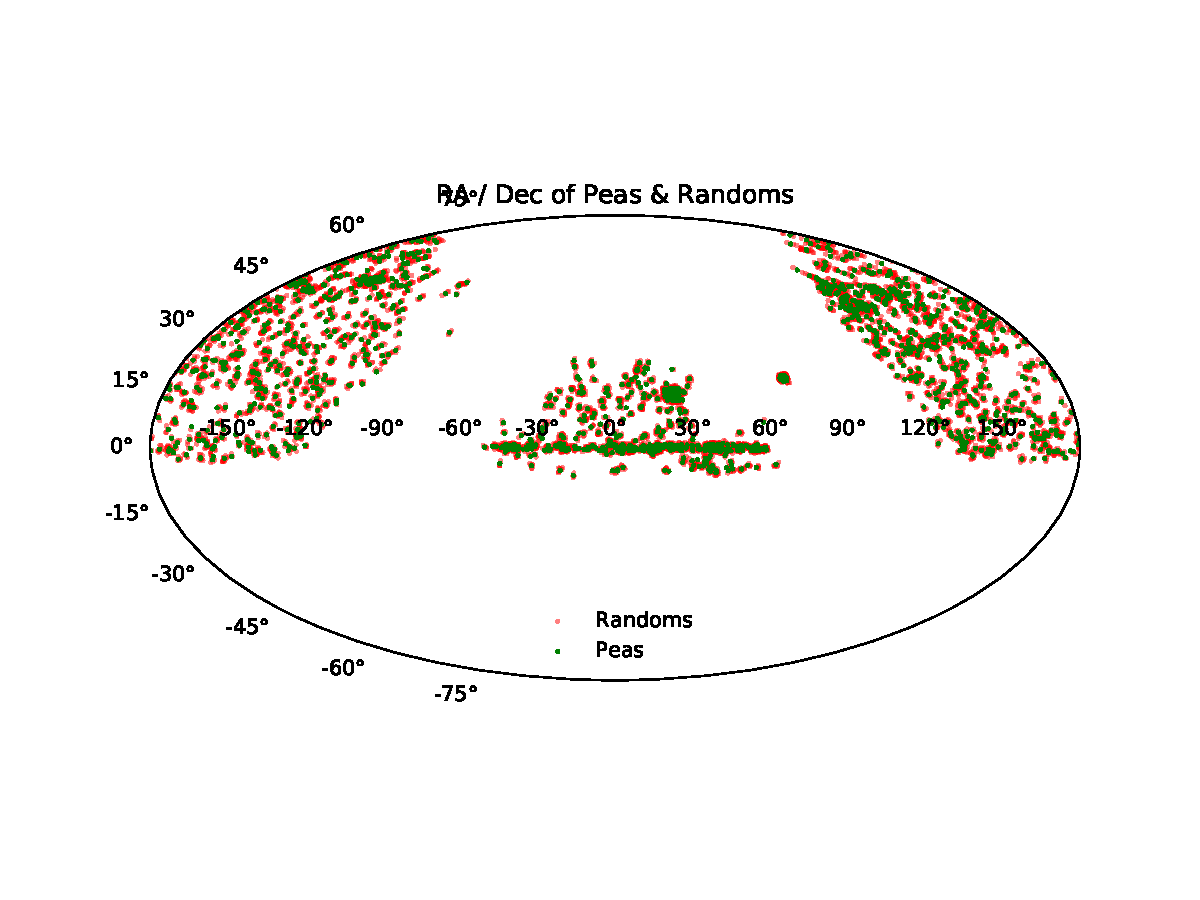
\includegraphics[width=1\textwidth, angle=0]{PeaRand_ra_dec.pdf}
\end{center}
\caption{\small{ Looking into redshift distribution of new Peas from DR12.  There are perhaps relatively more at lower $z<0.2$
}}
\label{fig:orig}
\end{figure}



\section{The original 80 }
Cardamone et al 2009 leveraged a sample of 251 colour-selected galaxies in SDSS DR7 between $0.112<z<0.360$ using a series of color cuts to define the original `pea' galaxies.
\begin{equation}
u-r \le2.5 \\
\end{equation}
\begin{equation}
r-i \le  -0.2 \\
\end{equation}
\begin{equation}
r-z \le 0.5 \\
\end{equation}
\begin{equation}
g-r \ge r-i+0.5 \\
\end{equation}
\begin{equation}
u-r \ge  2.5(r-z) \\
\end{equation}
Using the existing spectra, the sample was further refined to 80 objects that met a specific requirement of AON greater than 3 in each of the 4 line diagnostics in BPT diagram and falling into the star forming spectral line ratios.   This came from a sample of 103 narrow line objects with $S/N > 3$ in each of the lines of the BPT diagram.  One of the objects was a Broad-line AGN and 8 were Narrow Line Seyfert 1s, meaning that 112 out of the 251 galaxies had spectra that were classified in that original work.  This limited sample was followed up on in the paper as it's characteristics (including masses, metalicities and star formation rates were determined).  With that original sample from DR7, an attempt to estimate their environment was made selecting a sample of random galaxies matched in luminosity and redshift and comparing projected neighbors within a radius of 1Mpc brighter than an iBand magnitude of -20.5 (At the redshift of the target).  This initial test showed that the Peas inhabit significantly lower density regions than typical galaxies at the same i-band magnitude and a median environmental density surrounding them was less than 2/3rds that of normal galaxies.  In this memo, we will refer to this final sample of 80 object as the original pea galaxies.



\section{environments of the original peas}
\subsection{Searching for Neighbors}
At $z=0.275$, the median redshift of the original 80 peas, the angular scale distance is 871.7 Mpc, providing a scale of 4.226 kpc/" (Wright (2006, PASP, 118, 1711). % Angular scale Distance = size /angle [radians], so 871.7Mpc ~ 206265 arcseconds, 
Therefore, a galaxy of size 10 kpc would extend $~2.37$ arcseconds on an SDSS image at this redshift, and a group scale of 1 Mpc would extend 236" on the sky, and a large cluster on the scale of 10 Mpc would be 2366" or nearly 40' on the sky in diameter.
\begin{equation}
1" \times 0.004226 Mpc/" \\
\end{equation}

We started a simple search near the positions of each of the original 80 peas in the SDSS DR13 catalogs.  Searching within $\pm$ 1 Mpc in RA and DEC of the 80 pea's positions, the DR 13 photoobj all catalog had 107298 objects and the spectroscopic catalog had 38854 objects (at any redshift!).  All of the original 80 objects are returned in this search of the DR 13 catalog, although one near a saturated bright start has slightly different photometry.
Because the main photometric catalog contains many objects, most of which will turn out to be at other redshifts, we search the photometric redshift catalog for each of these objects. 
 It's also worth noting that fibre collisions on the same SDSS plate prevented fibers from being placed closer than 55 arcsec and can effect the density of objects with redshift measurements in any field.
 The photometric redshifts are calculated for all objects in the primary catalog tagged as galaxies using an empirical training set with a kd-tree nearest neighbor fit (Beck et al. in prep).  There are 18,505 objects with photometric redshifts or $17\%$ of the catalog.  However, of those objects only 4125 have reliable photometric redshifts with calculated uncertainties (less than $4\%$ of the sample).

Starting with this set of objects, we find the neighbors for each pea within a projected distance of 236 arcseconds on the image.  The number of neighbors for these peas range from just over 200 to 4000.  For the two peas in Stripe 82, with the deeper imaging, the neighbors are greater (8634 and 14742).
However, this suggests that these peas can be found in a variety of environments.

%Insert table of counts.


What would be most helpful, would be to select for objects near the redshift of the pea
But numbers vary with depth of image (not necessarily the physical space density, as can be seen with the Stripe  82 data).


\begin{figure}[h]
\begin{center} %NOTE compile with TEX & DVI
%\includegraphics[width=1\textwidth, angle=0]{pea_zdist.ps}
\end{center}
\caption{\small{ Looking into redshift distribution of new Peas from DR12.  There are perhaps relatively more at lower $z<0.2$
}}
\label{fig:orig}
\end{figure}


The original sample of 80 confirmed peas was derived from DR7 after fitting the spectra for BPT Star Forming Galaxies from a sample within the color space (above) and $0.112<z<0.360$, where the OIII line falls in the r-band filter.  The main goal of Cardamoneetal2009 was to select a uniform sample of objects that could be investigated to uncover their properties.  The redshift range was selected so that the OIII line fell within the r-band filter (providing the 'green' appearance in the SDSS images) and a color selection region was defined to avoid sequences of galaxies and QSOs.  There is no uniform selection for the objects throughout the SDSS footprint,  as we look for Peas only in the spectroscopic sample of objects and keep them only in objects with classified as Starforming with spectral line amplitude over noise (AON) $\ge 3$ in all 4 lines in the BPT diagnostic. 
 In this paper, our goal is to quantify the environments in which these galaxies live.  In order to study this we take advantage of the huge expansion of SDSS spectroscopy through DR13, and use this to expand our sample of Peas.   

Starting with the simple color-selection region within the redshifts $0.112<z<0.360$, DR13's PhotoObjAll catalog provides a sample of 4155 galaxies, which could be nominally labeled as 'pea' colored.  This sample also includes the requirement's of a PSFMAG\_R $\ge 10$ and PETRORAD\_R $\le 5$.  However, DR13's PhotoObjAll catalog contains numerous interloping objects (from artifacts, small regions of larger galaxies, and other objects with bad photometry).  We wish to again select a catalog of Star Forming Peas, compact and with OIII emission powered by star formation.  To recover this sample, we require spectral line measurements and therefor use the catalog provided by the Portsmouth Group in DR12, which uses the same programs we used for the original sample (Penalized PiXel Fitting (pPXF, Cappellari and Emsellem 2004) and Gas and Absorption Line Fitting code (GANDALF v1.5; Sarzi et al. 2006)) to derive emission line properties (Thomas et al. (2013) ). 

 Looking at images of the galaxies, shows many interloping objects which do not physically appear as peas.  Of the objects in the color-redshift space, 2203 have spectral fits in the Portsmouth catalog.   Many have non-starfomring BPT diagnostics, including 213 Seyfert galaxies, 65 LINERa, and another (52+103+87= 242) composite spectra.   Selecting for starforming objects only, leaves a sample of 1592 objects.  Requiring clean photometry (SDSS flag CLEAN=1, removing objects with deblending issues, those on plate edges, etc.), leaves 1454 objects. Of the 138 objects with the Clean flag =0, there are perhaps a dozen that look like clean peas on the image.  If we wish to limit the sample to those with individual $AON>3$ in each of the special line measurements, only 739 objects remain.  For the initial purposes of the clustering measurements - we'll use the full sample.


\begin{figure}[h]
\begin{center} %NOTE compile with TEX & DVI
%\includegraphics[width=1\textwidth, angle=90]{peaphotflag0.ps}
\end{center}
\caption{\small{ Phot Flag 0 sample of objects, removed from the spectroscopic sample eventhough classified as SF.  Of the 138 objects with the Clean flag ne 1, there are perhaps a dozen that look like clean peas on the image.  
}}
\label{fig:orig}
\end{figure}



% galaxies (or galaxies / peas)
%\begin{figure}[h]
%\begin{center} %NOTE compile with TEX & DVI
%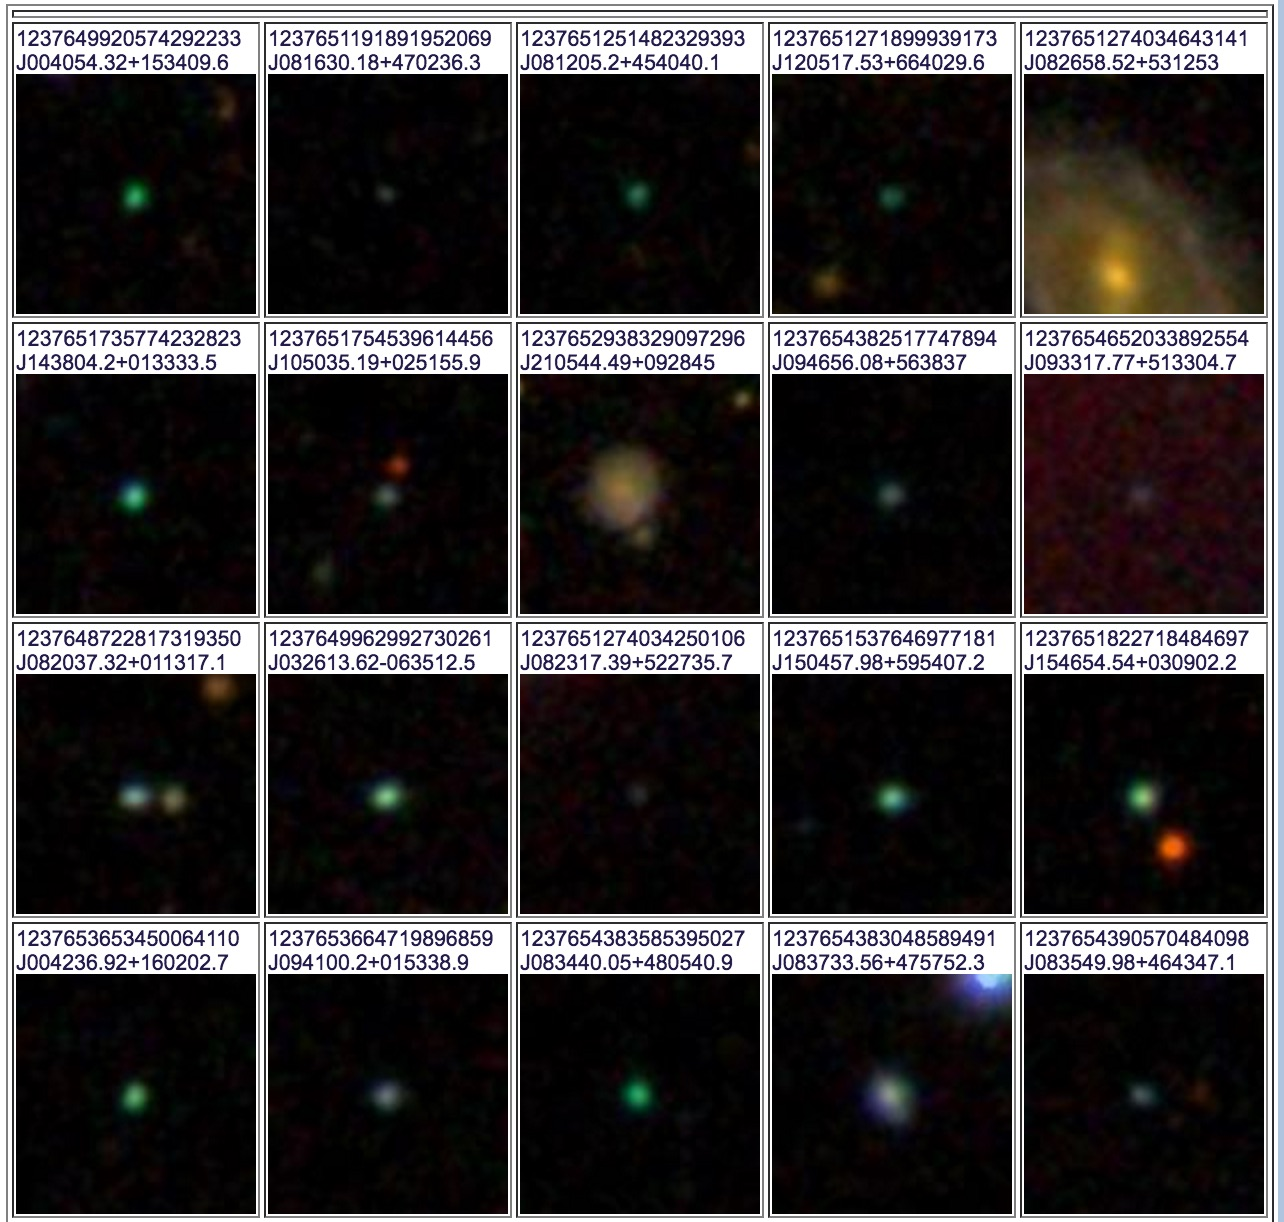
\includegraphics[width=1\textwidth, angle=0]{peaselectionsnapshot.jpg}
%\end{center}
%\caption{\small{ Figure 3 from Cardamone et al. 2009 (made by Stephen Bamford).  The cumulative distribution of neighbour counts for the Peas
%(solid line) is significantly different than a comparison galaxy sample (dotted line). No Peas live in the highest density environments.
%}}
%\label{fig:orig}
%\end{figure}



%\section{Figures}
%\begin{deluxetable}{l rl rl  rl}
%\tabletypesize{\scriptsize}
%\tablecolumns{7}
%\tablewidth{0pc}
%\tablecaption{Peas Hunts}
%\tablehead{
%\multicolumn{1}{c}{}
%&\multicolumn{2}{c}{\% of Spirals}
%&\multicolumn{2}{c}{\% of Non-Bar Spirals} 
% & \multicolumn{2}{c}{\% of Barred Spirals }\\
%%  \cline{6-13} \\ 
%%\colhead{Activity }
%%&\multicolumn{2}{c}{$9  < \log {\rm m} < 13$}
%%&\multicolumn{2}{c}{$9  < \log {\rm m} < 13$}
%%&\multicolumn{2}{c}{$9  < \log {\rm m} < 13$}
%%&\multicolumn{2}{c}{$9 < \log {\rm m} < 10$ }
%%&\multicolumn{2}{c}{$ 10  < \log {\rm m} < 11$}  
%%&\multicolumn{2}{c}{$ 11  < \log {\rm m} <  13$} \\
%\colhead{ }
%&\multicolumn{2}{c}{(1)}
%&\multicolumn{2}{c}{(2)}
%&\multicolumn{2}{c}{(3)}
%}
%\startdata
%            SF &  4791 &   0.45  &  3524 &   0.49 &      1267 &   0.39 \\
%\tableline
%            Sum & 10552 &   1.00  &  7262 &   1.00 &      3290 &   1.00 \\
%\enddata
 %\tablecomments{This table lists the number of galaxies in the sample, separated by activity type as determined from the BPT diagram: Star Forming, Transition Objects, AGN, LINER or Quiescent (meaning no strong emission lines).  The sample is then split into galaxies with-out bar features (Column 2) and those with identified bar features (Column 3).  In each case the number of galaxies is followed by the fraction of the sample that number represents.}
% \label{tab:type}
%\end{deluxetable}


%\begin{figure}[h]
%\begin{center}
%\includegraphics[width=0.49\textwidth]{colmassspiralagn.ps}
%\includegraphics[width=0.49\textwidth]{colmassbars.ps}
%\end{center}
%\caption{\small{The population of face-on spirals peaks in the most massive blue galaxies, but the highest fraction of these galaxies with bars occurs at redder colors. 
%The population of AGN peaks in the most massive green galaxies, and the fraction of these galaxies with bars is slightly larger than that of the general galaxy population  (top right).
%}}
%\label{fig:cmas}
%\end{figure}

%\section{Acknowledgements}
%Funding for the SDSS and SDSS-II has been provided by the Alfred
%P. Sloan Foundation, the Participating Institutions, the National
%Science Foundation, the U.S. Department of Energy, the National
%Aeronautics and Space Administration, the Japanese Monbukagakusho, the
%Max Planck Society, and the Higher Education Funding Council for
%England. The SDSS Web Site is http://www.sdss.org/.

%The SDSS is managed by the Astrophysical Research Consortium for the
%Participating Institutions. The Participating Institutions are the
%American Museum of Natural History, Astrophysical Institute Potsdam,
%University of Basel, University of Cambridge, Case Western Reserve
%University, University of Chicago, Drexel University, Fermilab, the
%Institute for Advanced Study, the Japan Participation Group, Johns
%Hopkins University, the Joint Institute for Nuclear Astrophysics, the
%Kavli Institute for Particle Astrophysics and Cosmology, the Korean
%Scientist Group, the Chinese Academy of Sciences (LAMOST), Los Alamos
%National Laboratory, the Max-Planck-Institute for Astronomy (MPIA),
%the Max-Planck-Institute for Astrophysics (MPA), New Mexico State
%University, Ohio State University, University of Pittsburgh,
%University of Portsmouth, Princeton University, the United States
%Naval Observatory, and the University of Washington.

%\bibliographystyle{/Users/cnc/Documents/Yale/write/bibtex/apj}
%\bibliographystyle{/Users/cnc/Documents/Yale/write/bibtex/mn2e}

\bibliographystyle{mnras}
%\bibliographystyle{mn}
%\bibliography{/Users/cnc9/Documents/Yale/write/bibtex/apj-jour,/Users/cnc9/Documents/Yale/write/bibtex/refs}
\bibliography{refs}

\end{document}
